% Figure 1: the model. (A) The life cycle of species i in patch x during one
% time step. (B) The conditions theta_x(t) that set reproduction, in five
% asynchronous patches, for predictable variation and red noise.
%
% Panel B is drawn by analysis/env_time_series.R, which must be run first.
%
% The schematic follows the order of the life cycle in
% simulations/metacom_regimes.R and the manuscript, in taxon-neutral terms
% (seeds, eggs, or spores are all propagules): (1) emergence splits the
% propagule pool into active individuals and dormant propagules, and the
% community is censused; (2) active individuals reproduce, limited by the
% environment and by competition; (3) dormant propagules survive in the bank;
% (4) new propagules disperse, and the arriving propagules and the surviving
% dormant propagules are the propagule pool of the next step. Solid arrows are
% flows of propagules or individuals; dashed arrows carry
% information (the cue) or conditions (the environment). Grey italic labels name
% the distribution of each random draw: demographic stochasticity.
%
% Compile from the repository root:
%   latexmk -pdf -jobname=model -outdir=figures/main \
%     -auxdir=analysis/build analysis/model_figure.tex

\documentclass[border=4pt]{standalone}
\usepackage{amsmath}
\usepackage[scaled]{helvet}
\usepackage[T1]{fontenc}
\renewcommand{\familydefault}{\sfdefault}
\usepackage{sansmath}
\sansmath
\usepackage{graphicx}
\usepackage{tikz}
\usetikzlibrary{arrows.meta, positioning, calc}

% Colors: soil band and the information arrows stay readable in grey scale
\definecolor{soil}{gray}{0.92}
\definecolor{info}{gray}{0.40}

% The distribution of each random draw, set under its rate
\newcommand{\dist}[1]{{\itshape\color{info}#1}}

\begin{document}
\begin{tikzpicture}[
    font=\footnotesize,
    stock/.style={draw, rounded corners=2pt, fill=white, align=center, inner xsep=2pt,
                  minimum width=2.6cm, minimum height=1.0cm, line width=0.6pt},
    elsewhere/.style={stock, dashed},
    flow/.style={-{Stealth[length=2.2mm]}, line width=0.8pt},
    signal/.style={-{Stealth[length=1.8mm]}, dashed, color=info, line width=0.6pt},
    process/.style={font=\footnotesize\bfseries, align=center},
    rate/.style={font=\footnotesize, align=center},
  ]

  % --- panel labels -------------------------------------------------------------------
  \node[anchor=north west, font=\normalsize\bfseries] at (-1.5, 4.6) {A};
  \node[anchor=north west, font=\normalsize\bfseries] at (-1.5, -4.7) {B};

  % --- (B) conditions through time, drawn by analysis/env_time_series.R ----------------
  \node[anchor=north west, inner sep=0pt] at (-1.5, -5.2)
    {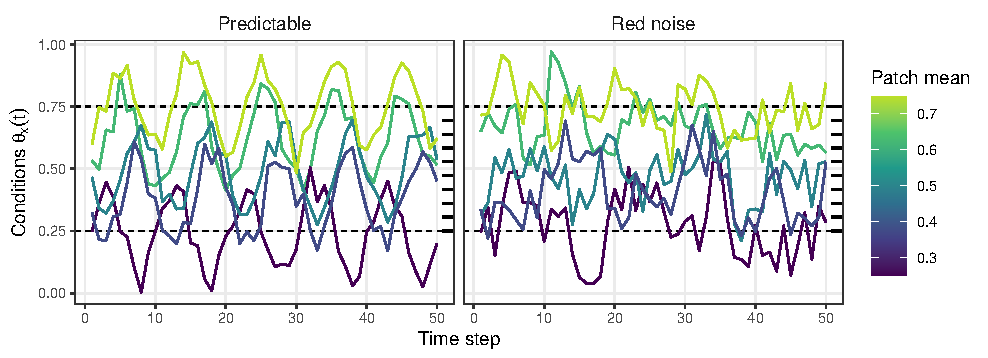
\includegraphics{figures/main/panels/env_asynchronous.pdf}};

  % --- the active habitat and the bank ------------------------------------------
  % 16.75 cm wide, so the figure prints at full page width (173 mm) without scaling
  \fill[soil] (-1.5, 0) rectangle (15.25, -4.3);
  \draw[line width=0.6pt] (-1.5, 0) -- (15.25, 0);
  \node[anchor=south west, color=info] at (0.1, 0.05) {Active habitat};
  \node[anchor=north west, color=info] at (0.1, -0.05) {Seed bank};

  % --- state variables ---------------------------------------------------------
  \node[stock] (P)  at (0, -1.6)     {Propagule pool\\ $P_{ix}(t)$};
  \node[stock] (G)  at (3.9, 2.0)    {Active individuals\\ $A_{ix}(t)$};
  \node[stock] (D)  at (3.9, -1.6)   {Dormant propagules\\ $D_{ix}(t)$};
  \node[stock] (B)  at (9.2, 2.0)    {Propagules\\ produced $B_{ix}(t)$};
  \node[stock] (Ds) at (9.2, -1.6)   {Surviving dormant\\ propagules $D^{\ast}_{ix}(t)$};
  \node[stock] (R)  at (13.55, -1.6) {Arriving propagules\\ $R_{ix}(t+1)$};
  \node[elsewhere] (Y) at (13.55, 2.0) {Other patches\\ $y$};

  % --- census: once per step, after emergence --------------------------------
  \draw[densely dotted, line width=0.7pt] (5.45, 3.85) -- (5.45, -2.75);
  \node[anchor=south] at (5.45, 3.85) {Census};

  % --- (1) emergence ------------------------------------------------------------
  \draw[flow] (P.north) |- (G.west);
  \node[process, anchor=south] at (1.2, 2.05) {(1) Emerge};
  \node[rate, anchor=north] at (1.2, 1.92) {$g_{ix}(t)$\\ \dist{binomial}};
  \draw[flow] (P.east) -- node[rate, below=1pt] {$1 - g_{ix}(t)$} (D.west);

  % the cue that sets the emergence probability
  \node[rate, color=info, anchor=south] (cue) at (2.25, 3.05)
    {$\operatorname{logit} g_{ix}(t) = b_i + \beta\,\tilde c_{ix}(t)$};
  \draw[signal] (cue.south) -- (2.25, 2.1);

  % --- (2) reproduction ---------------------------------------------------------
  \draw[flow] (G.east) -- node[process, above=1pt] {(2) Reproduce}
    node[rate, pos=0.56, below=2pt] {$\dfrac{f_i(\theta_x(t))}{1 + \sum_j \alpha_{ji} A_{jx}(t)}$\\ \dist{Poisson}}
    (B.west);

  % the environment that sets reproduction
  \node[rate, color=info, anchor=south] (env) at (7.75, 3.05) {Conditions $\theta_x(t)$};
  \draw[signal] (env.south) -- (7.75, 2.1);

  % --- (3) survival in the bank -----------------------------------------------------------------
  \draw[flow] (D.east) -- node[process, above=1pt] {(3) Survive}
    node[rate, below=1pt] {$s$\\ \dist{binomial}} (Ds.west);

  % --- (4) dispersal ---------------------------------------------------------------------
  \draw[flow] (B.east) -- node[process, above=1pt] {(4) Emigrate}
    node[rate, below=1pt] {$m$\\ \dist{binomial}} (Y.west);
  \draw[flow] (B.south east) -- node[rate, pos=0.3, below left=0pt] {$1 - m$} (R.north west);
  \draw[flow] (Y.south) -- node[rate, pos=0.3, right=1pt, align=left] {Immigrate\\ $K_{xy}$\\ \dist{multinomial}} (R.north);

  % --- the next time step ----------------------------------------------------------------
  \draw[flow] (R.south) |- (5.0, -3.55) -| (P.south);
  \draw[line width=0.8pt] (Ds.south) -- (Ds.south |- 0, -3.55);
  \node[rate, fill=soil, anchor=north] at (6.6, -3.6)
    {Next step: $P_{ix}(t+1) = R_{ix}(t+1) + D^{\ast}_{ix}(t)$};

\end{tikzpicture}
\end{document}
